\chapter{Introduction}
\section{Water Cycle}
Water is one of the most necessary resources for human beings. It is the most important ingredient of life; it has a regulating effect on climate and all industries can not function well without it. However, 98 \%
of the water on the earth is in the oceans, 1.6\% is in ice caps, which means only 0.4 \% is the
fresh water on land. So, a very little variability of the hydrology cycle can have big effects on
water resources. \\\\
The hydrology cycle (see figure \ref{fig:hydrologic cycle}) includes 3 major parts: evaporation, precipitation and runoff. The water evaporates from the oceans and the land surface as vapor to become part of the atmosphere along with water from evapotranspiration, which is water transpired from plants and evaporated from the soil and the cooler temperature causes the vapor into clouds. The clouds fall out of the sky as precipitation, which includes rain, snow and ice. Most precipitation falls back into the oceans or onto land. Precipitated water may be intercepted by vegetation, become overland flow over the ground surface, flow through the soil as subsurface flow and discharge into streams as surface runoff. The process can be simplified as:
\begin{equation}
	\frac{dS}{dt} = Pre - ET - R
\end{equation}
where
\begin{table}[htbp]
	\begin{tabular}{ll}
		$Pre$   & Precipitation    \\ 
		$ET$    & Evatranspiration \\ \
		$R$     & Surface Runoff \\ 
		$dS / dt$ & total water storage change \\ 
	\end{tabular}
\end{table}
\begin{figure}[htbp]
	\centering
	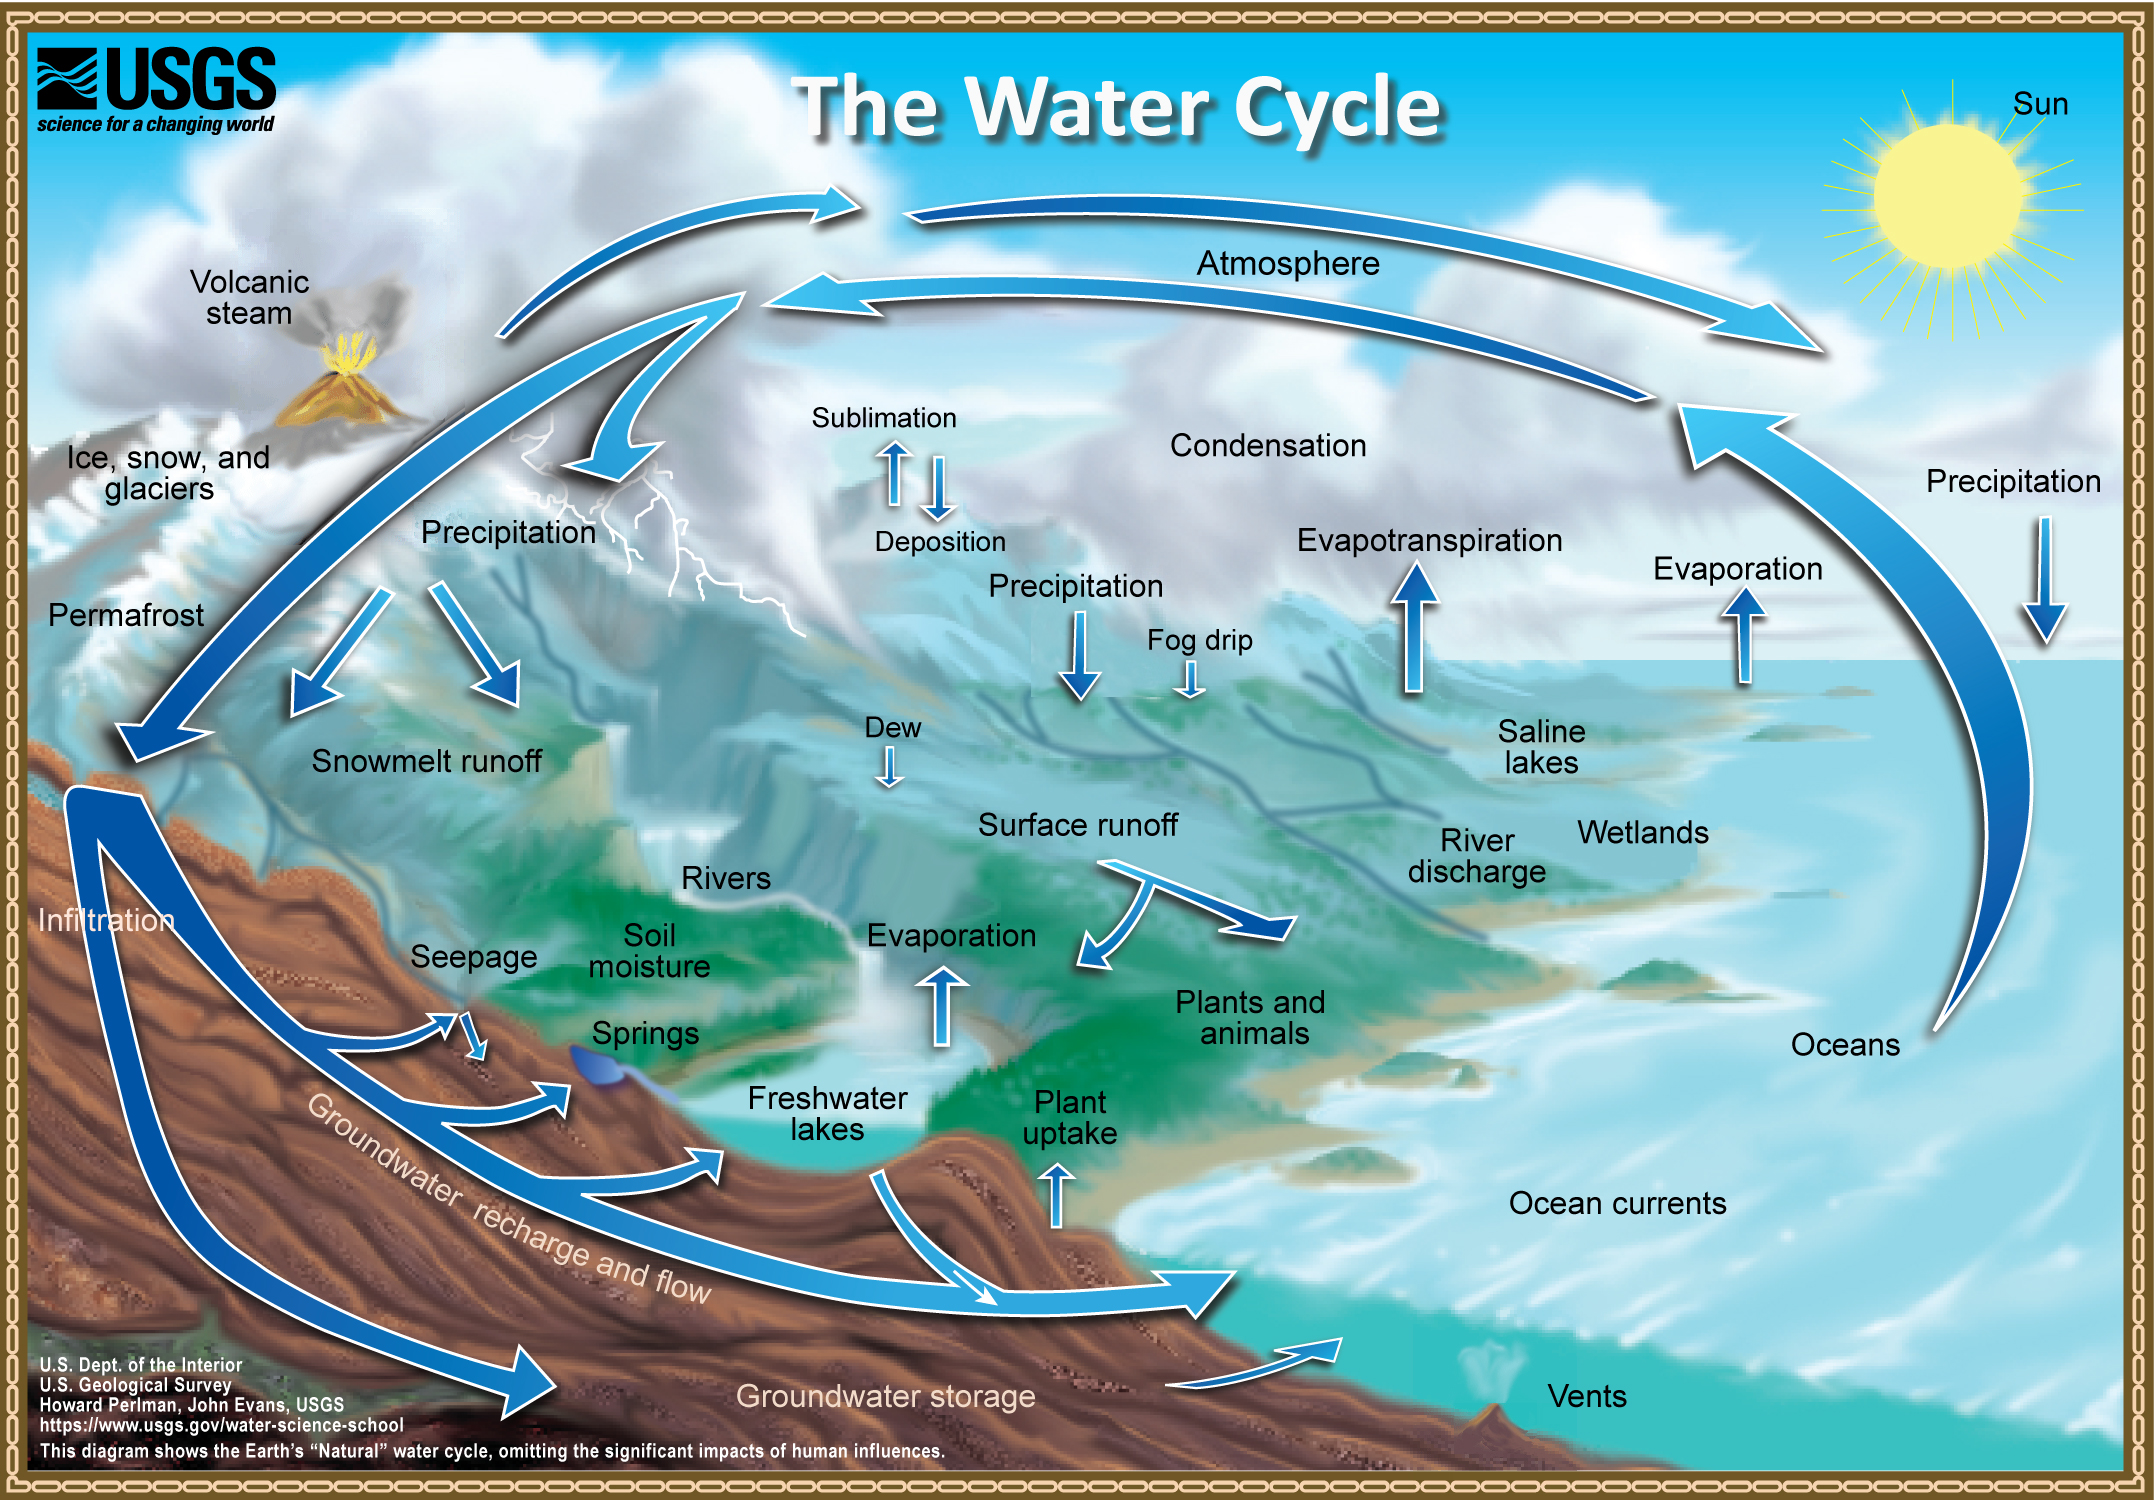
\includegraphics[width=0.7\textwidth]{water-cycle-natural} % Datei in "bilder/" bei LaTeX: eps, bei PDFLaTeX: jpg (o.ä.) 
	\caption{Horologic Cycle} 
	\label{fig:hydrologic cycle}
\end{figure}
\section{Observation from Satellite}
It was extremely difficult to measure the global water storage change consistently. In some way, remote sensing with satellite is the perfect tool for hydrology research, which has the ability to provide the data globally in a long term.\\\\
The GRACE twin satellites, launched 17 March 2002, are making detailed measurements of Earth's gravity field, which are caused by monthly changes in mass. The mass changes can be thought of as concentrated in a very thin layer of water thickness changes near the Earth's surface by moving ocean, atmospheric and land ice masses and by mass exchanges between these Earth system compartments. \\\\
There are 2 satellites with tandem polar orbit. Since the orbit is around the pole and the earth rotates itself, the satellites were able to get the whole view of the earth. Unlike the normal remote sensors, the GRACE satellites measured the gravity field of the earth. When the 2 satellites went over a mass anomaly like a big mountain, the distance of them will be a little bit smaller. By calculating this distance difference with the help of GPS system, the gravity field anomaly of the earth along with the total water storage anomaly are able to be plotted monthly. \\\\
It is shown, that GRACE delivers the highest temporal resolution and is thus able to observe monthly mass variation with a spatial resolution of less than 1000\ut{km}. In (Wahr et al., 1998) it was predicted that GRACE would be able to measure these effects with an accuracy of about 2\ut{mm} of water equivalent heights. Though this accuracy has not yet been achieved because of the errors in spherical harmonic coefficients of short-wavelength, it was shown in many publications that the Stokes coefficients from GRACE indeed contain hydrological signals as the monthly solutions from GRACE showed a good agreement with mass variations from hydrological models.
\begin{figure}[htbp]
	\centering
	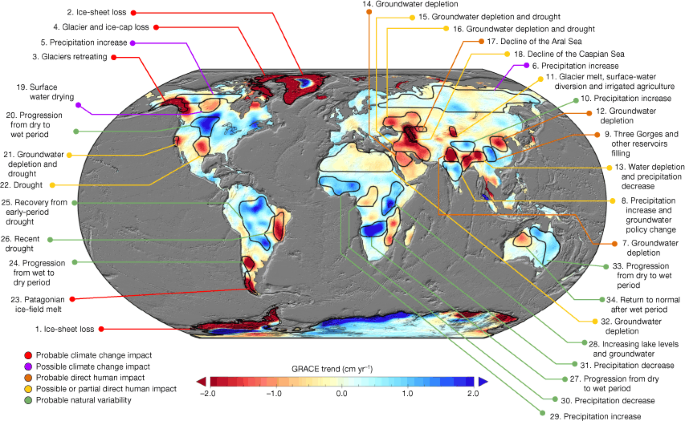
\includegraphics[width=0.6\textwidth]{TWSA} % Datei in "bilder/" bei LaTeX: eps, bei PDFLaTeX: jpg (o.ä.) 
	\caption{Water Storage Change} 
	\label{fig:TWSA}
\end{figure}
\begin{figure}[ht]
	\centering
	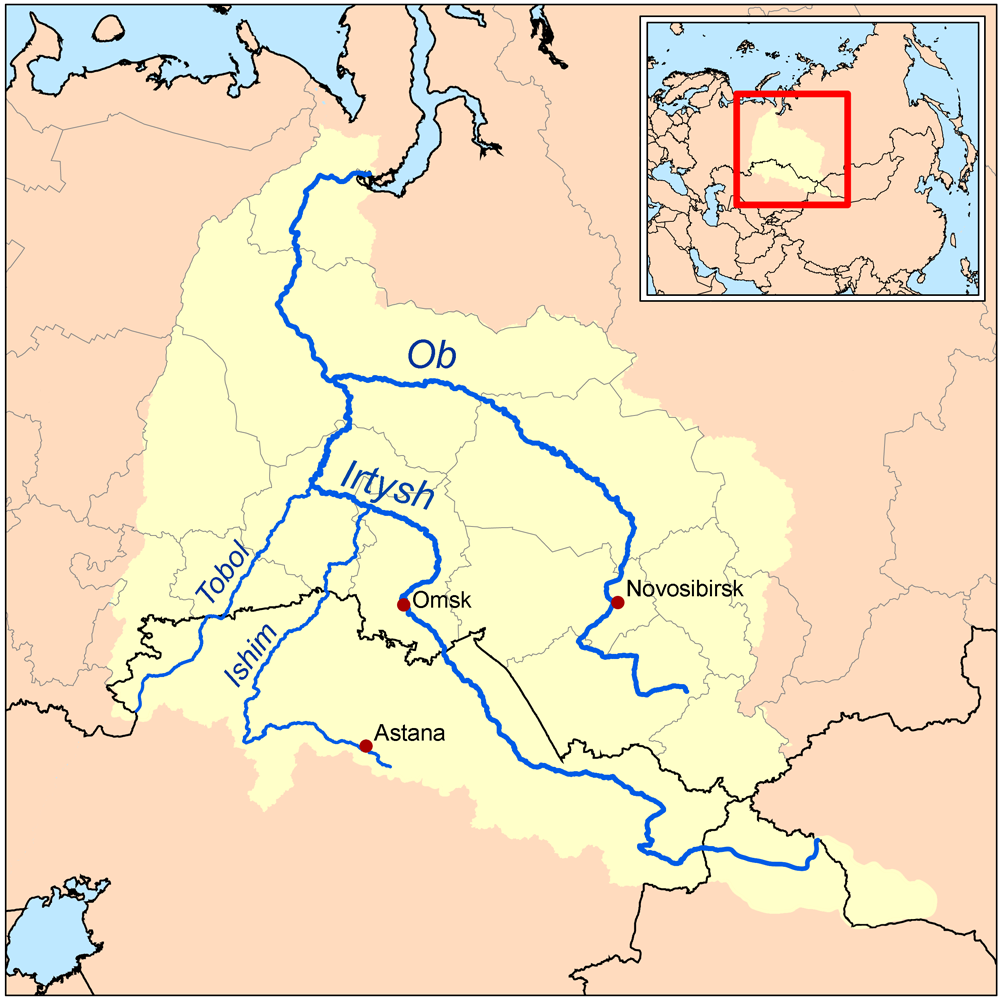
\includegraphics[width=0.6\textwidth]{Obbasin} % Datei in "bilder/" bei LaTeX: eps, bei PDFLaTeX: jpg (o.ä.) 
	\caption{Ob basin} 
	\label{fig:Obbasin}
\end{figure}\\
\section{Motivation}
A time series is a series of data points indexed (or listed or graphed) in time order. Most commonly, a time series is a sequence taken at successive equally spaced points in time. Thus it is a sequence of discrete-time data.  In hydrology, most variables are observed in time series, including Total Water Storage Anomaly(TWSA). In the hydrological cycle, this should reflect seasonal behavior and is in long term relatively stable. However, it was shown that since 2002 the TWSA of many big basins has increased (see figure \ref{fig:TWSA}). One important basin of them is Ob basin in west Siberia (see figure \ref{fig:Obbasin}). How did this trend happen is a very interesting topic. Through the analysis of the trend of the time series, it is possible to further understand the changes that have taken place before and future changes can also be predicted based on the stationary analysis.
\section{Objective}
In this thesis, the beginning point of the changing trend is to be found by analyzing the TWSA time series from GRACE data. In order to find the reason of the change, the precipitation, the evatranspiration along with the runoff in the same period from different data center would also be processed and compared with the TWSA. At the end, how was the changes of the TWSA and the reasons for this change would be discussed. 
